\documentclass{kththesis}

\usepackage{blindtext} % This is just to get some nonsense text in this template, can be safely removed

\usepackage{csquotes} % Recommended by biblatex
\usepackage{biblatex}
\addbibresource{references.bib} % The file containing our references, in BibTeX format

% Own packages -------------------------------------
\usepackage{graphicx}
\graphicspath{ {images/} }
\usepackage{amsfonts}
\usepackage{amsmath}
\usepackage[acronym]{glossaries}
\usepackage{algorithm,algorithmic}% http://ctan.org/pkg/algorithms
\makeglossaries
\newacronym{gan}{GAN}{Generative Adversarial Network}
\newacronym{gans}{GANs}{Generative Adversarial Networks}
\newacronym{vae}{VAE}{Variational Autoencoder}
\newacronym{vaes}{VAEs}{Variational Autoencoders}
\newacronym{mse}{MSE}{Mean Squared Error}
\newacronym{aevb}{AEVB}{Auto Encoding Variational Bayes}
% --------------------------------------------------
% Own commands ---------
\newcommand{\ve}[1]{\mathbf{#1}}
\newcommand{\dataset}{\mathcal{S}}
\newcommand{\latentspace}{\mathcal{Z}}
\newcommand{\dataspace}{\mathcal{X}}
% ----------------------

\title{High Quality Synthetic Data Generation with Semi-Supervised Adversarial Networks}
\alttitle{Neurala Nätverk för Högkvalitativ Syntetisk Datagenerering}
\author{Mårten Nilsson}
\email{marten3@kth.se}
\supervisor{Josephine Sullivan}
\examiner{Hedvig Kjellström}
\programme{Master in Machine Learning}
\school{School of Computer Science and Communication}
\date{\today}


\begin{document}

% Frontmatter includes the titlepage, abstracts and table-of-contents
\frontmatter

\titlepage

\begin{abstract}
  English abstract goes here.

  \blindtext
\end{abstract}


\begin{otherlanguage}{swedish}
  \begin{abstract}
    Träutensilierna i ett tryckeri äro ingalunda en oviktig faktor,
    för trevnadens, ordningens och ekonomiens upprätthållande, och
    dock är det icke sällan som sorgliga erfarenheter göras på grund
    af det oförstånd med hvilket kaster, formbräden och regaler
    tillverkas och försäljas Kaster som äro dåligt hopkomna och af
    otillräckligt.
  \end{abstract}
\end{otherlanguage}

\section*{Acknowledgements}
Josephine Sullivan, Hedvig Kjellström, Alexander Davies, Family and Friends etc. 

\tableofcontents


% Mainmatter is where the actual contents of the thesis goes
\mainmatter

% Here's my thesis ---------------------------------------------------------------------------------------

\chapter{Introduction}
Motivation: Data compresion, can express data sets with smaller space requirements. Improved consistency (better annotations). Semi-supervised learning. Implicit semi-supervised learning.

Establish the context and importance of the topic in this text.

\section{Motivation for synthetic data generation}

\section{Problem statement}

\section{Scope and objectives}

\section{Thesis overview}
Chapter 2 provides and overview of \acrlong{gans} and related methods. The notation used throughout the thesis is establised in section 2.1. In Chapter 3, the method is presented etc...

\subsection{Semi-supervised learning}

\subsection{Data compression}




\chapter{Background}
This chapter begins by establishing the notation and the concepts that are encountered in this chapter. Thereafter a brief overview of generative models is provided. This is followed by an in-depth descriptions of the families of generative modells considered in this project. Finally the concept of semi-supervised learning is introduced.

\section{Concepts and Terminology}
%This chapter deals with high dimensional spaces (written in mathcal, $\mathcal{Z}$), stochastic variables (written in uppercase $Z$), sets (alsa mathcal), vectors (written as plain variables $z$) and probability distributions (reserving the letter $p$ for this, using indexes to distinguish different distributions).
This chapter deals with high dimensional spaces, stochastic variables, sets, vectors and probability distributions. Spaces and sets are written in mathcal ($\mathcal{Z}$), stochastic variables are written as uppercase letters ($Z$), vectors are written as lower case letters ($z$) and the letter $p$ is reserved for probabilities and probability distributions.

\section{Generative models}
\begin{figure}[t]
    \centering
    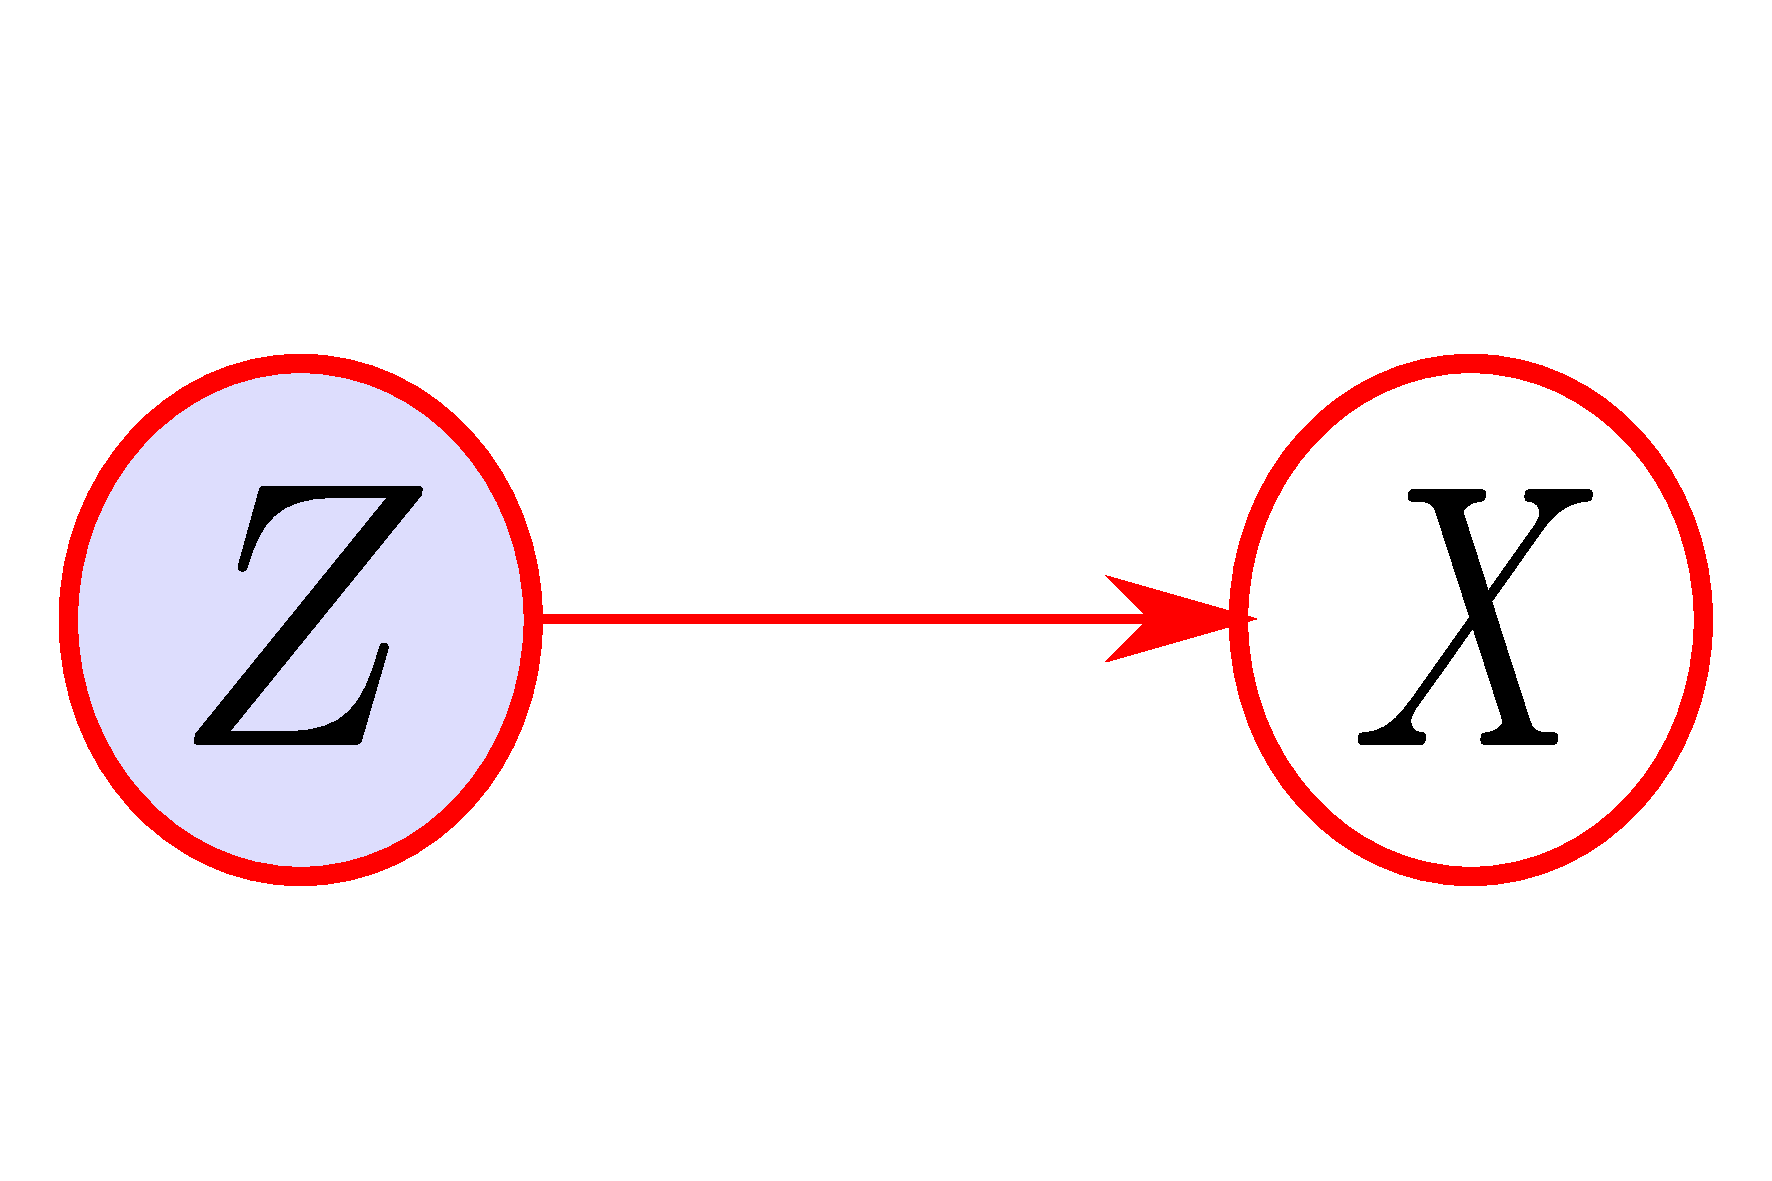
\includegraphics[width=0.5\textwidth]{graphicalModel.pdf}
    \caption{The directed graphical model representing the dependency between the latent variable $Z$ and the data variable $X$ in \acrshort{gans}. This is the same dependency structure as in GMMs and \acrshort{vaes}.}
    \label{fig:GANgraph}
\end{figure}
In this thesis, the term generative model refers to models that explicitly or implicitly represent the data distribution thereby allowing sampling from the modelled distribution. This is different from discriminative models which only model information that can be extracted from the data. 

<<<<<<< HEAD
This thesis focuses on parametric generative models which gan be formulated as instances of probabilistic graphical models \parencite{christopher2016pattern}. Examples of these include Gaussian Mixture Models (GMMs), Hidden Markov models (HMMs), \acrfull{gans} and \acrfull{vaes}. The attention of this work is directed towards models that are applicable on large, high-dimensional and complex data sets. The known models with these properties are  \acrshort{gans} and \acrshort{vaes}. Both of these assume a dependency between a latent variable $Z$ and an observed variable $X$ according to figure \ref{fig:GANgraph}. The rest of this chapter provides a more in-depth description of these models. 
=======
This thesis focuses on parametric generative models which can be formulated as instances of probabilistic graphical models \parencite{christopher2016pattern}. Examples of these include Gaussian Mixture Models, Hidden Markov models, \acrfull{gans} and \acrfull{vaes}. The attention of this work is directed towards models that are computationally tractable on large, high-dimensional and complex data sets. The known models with these properties are  \acrshort{gans} and \acrshort{vaes}. Both of these assume a casual dependency between a latent variable $Z$ and an observed variable $X$ according to figure \ref{fig:GANgraph}. The rest of this chapter provides a more in-depth description of these models. 
>>>>>>> 4886d906f95b333ed286f024e531f582fb58fd74

%Write short state of generative models. Boltzmann machine, explicit models, variational autoencoders etc...

\section{\acrlong{gans}}

\begin{figure}
    \centering
    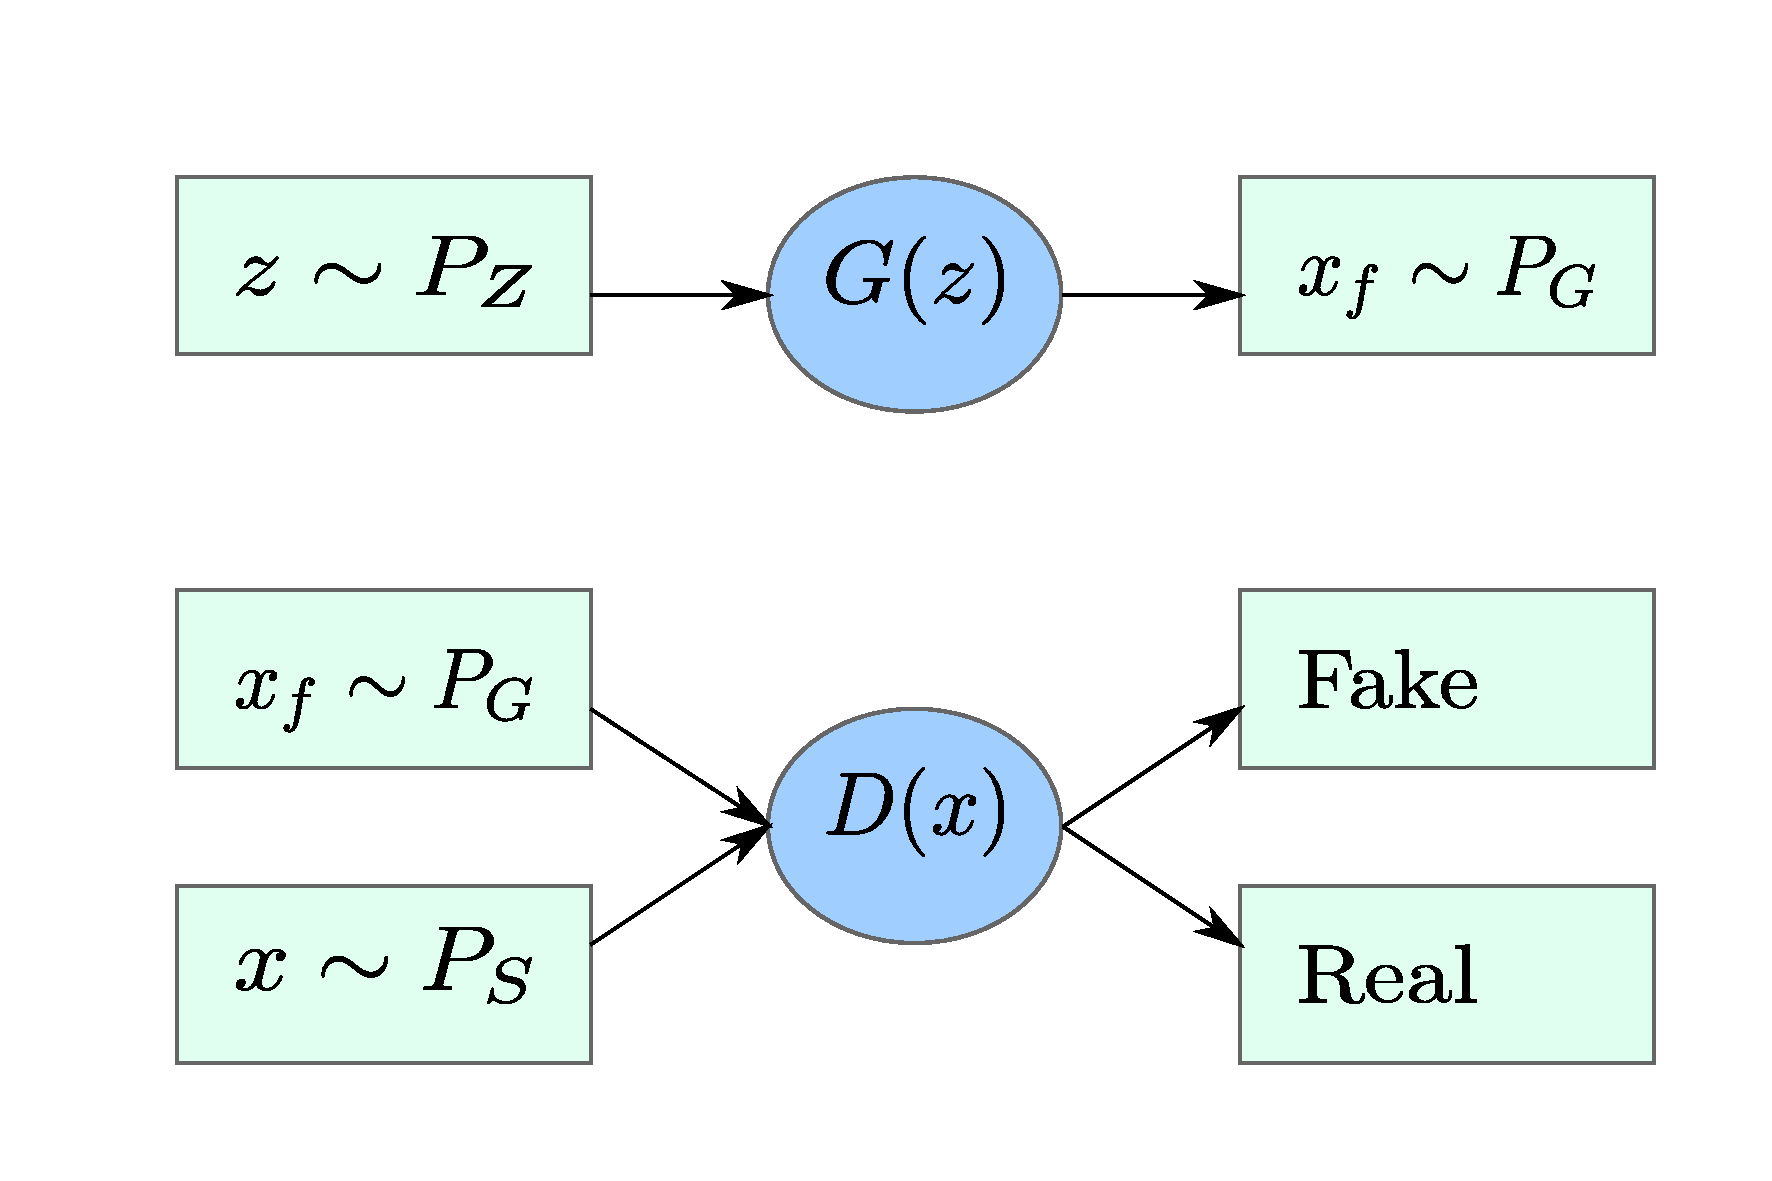
\includegraphics[width=\textwidth]{GANcomponents.pdf}
    \caption{The main components of \acrshort{gans}}
    \label{fig:GAN}
\end{figure}

\acrfull{gans} are a family of generative models proposed by \textcite{goodfellow2014generative}. The framework for training \acrshort{gans} consists of a data set $\dataset$ with elements in a domain $\dataspace$, a latent space $\latentspace$ and two neural networks, a generator $G(z)$ and a discriminator $D(x)$ (figure \ref{fig:GAN}). The generator maps elements of $\latentspace$ to $\dataspace$, $G: \latentspace \rightarrow \dataspace$. The discriminator is a binary classifier $D: \dataspace \rightarrow [0, 1]$. 

The objective of the discriminator is to classify elements in $\dataspace$ as either members or not members of $\dataset$. Members of $\dataset$ are usually referred to as real samples since they are part of the data set, and non-members are referred to as fake samples. The objective of the generator is to fool the discriminator by mapping elements in $\latentspace$ to the subspace of $\dataspace$ that is classified as real. 

The generator can be viewed as representing a probability distribution $p_G$ on $\dataspace$. By introducing a latent random variable $Z$ with the probability distribution $p_Z$ on $\latentspace$, the generator probability distribution can be expressed as $p_G(x) = p_Z(G^{-1}(x))$. 

In practice $G^{-1}$ is intractable to compute, whereby explicit probabilities are seldom acquired through \acrshort{gans}. However, this formulation allows sampling from the learned distribution as $G(z), z \sim p_Z$ is straightforward to compute. 

The goal of training \acrshort{gans} is to learn a probability distribution over the data. By viewing the elements of $\dataset$ as outcomes of a random variable $S$ with probability distribution $p_S$ the goal of the generator is to approximate this distribution with $p_G$, and the goal of the discriminator is to discriminate between these distributions. Using this formulation the objective of the \acrshort{gan} training can be formulated as a minimax game 
\begin{equation}
    \min_G \max_D -J^{D}(G, D)
\end{equation}
where $J^D(G, D)$ is the discriminator cost function from \parencite{goodfellow2016nips},
\begin{equation}
    J^D(G, D) = -\frac{1}{2}\mathbb{E}_{x \sim p_S, z \sim p_Z}\left[\log(D(x)) + \log(1 - D(G(z))) \right].
    \label{eq:GANcost}
\end{equation}
%\begin{equation}
%    \mathcal{L}(x_1, x_2) = -\log(D(x)) + \log(D(x_2)), \quad \begin{cases} x \in X \\ z \in \latentspace \end{cases}.
%\end{equation}
Since both the generator and discriminator are differentiable functions, (\ref{eq:GANcost}) can be optimized using standard gradient based optimization schemes such as RMSprop \parencite{tieleman2012lecture} or Adam \parencite{kingma2014adam}. Typically the networks are updated in an alternating fashion where the parameters of one of the networks are frozen while updating the other network. The expectectations in (\ref{eq:GANcost}) are typically estimated using minibatches as 
\begin{equation}
    \mathbb{E}_{x\sim p(x)}[f(x)] \approx \frac{1}{m}\sum_{i=1}^mf(x_i)
\end{equation}
where $x_i$ is sampled from $p(x)$. This process is described in an algorithmic fashion in Algorithm \ref{alg:GANbase}.


\begin{algorithm}
    \caption{Training scheme for \acrlong{gans} using minibatch stochastic gradient based optimization and $n_D$ discriminator updates per generator update. $\theta_D$ denotes the discriminator parameters and $\theta_G$ denotes the generator parameters.}
    \label{alg:GANbase}
    \begin{algorithmic}[1]
        \FOR{number of iterations}
        \FOR{$n_D$ steps do}
        \STATE sample minibatch of fake data $\{x_{f1}, ..., x_{fm}\} \sim p_G(x)$.
        \STATE sample minibatch of real data $\{x_{1}, ..., x_{m}\} \sim p_S(x)$.
        \STATE update discriminator parameters with the estimated gradient of the cost function
        \begin{equation}
            \nonumber
            \nabla_{\theta_D} \left( -\frac{1}{m}\sum_{i=1}^m\log(D(x_i)) + \log(1-D(x_{fi})) \right).
        \end{equation}
        \ENDFOR
        \STATE sample minibatch of fake images $\{x_{f1}, ..., x_{fm}\} \sim p_G(x)$.
        \STATE update generator parameters with the estimated gradient of the negative cost function
        \begin{equation}
            \nonumber
            \nabla_{\theta_G} \left( - \frac{1}{m}\sum_{i=1}^m\log(1-D(x_{fi})) \right).
        \end{equation}
        \ENDFOR
    \end{algorithmic}
\end{algorithm}


\subsection{Theoretical properties of \acrshort{gans}}
In the original paper (\textcite{goodfellow2014generative}) a couple of theoretical properties of \acrshort{gans} are formulated and proved. These proofs assume that both the generator and discriminator have infinite capacity.

Firstly it is proven that given a fixed generator $G$ the optimal discriminator is 
\begin{equation}
    D(x) = \frac{p_S(X=x)}{p_S(X=x) + p_G(X=x)}.
\end{equation}
A straightforward implication of this is that when $G$ is optimal, the optimal $D$ always output $0.5$ for all real and fake data points. In other words
\begin{equation}
    p_G \eqdist p_S \implies D(x) = 0.5 \; \forall x \sim p_G, p_S
\end{equation}
if $D$ and $G$ are optimal. Secondly, it is also proved in the original paper that given an optimal discriminator there exists a global maximum of the discriminator cost function and it is reached if and only if $p_G \eqdist p_S$. Finally convergence of the training algorithm (Algorithm \ref{alg:GANbase}) is also proven.

This means that one can observe convergence when training \acrshort{gans} by observing the discriminator output. When it saturates at $0.5$ for all generator samples and real samples the algorithm has converged. In practice it is difficult to get to this point with complex sets of high-dimensional data.

\subsection{Practical issues}
The theoretical properties indicate that \acrshort{gans} are a sensible method for implicitly learning probability distributions. However when implementing these models in practice some issues emerge from using models of finite capacity. 

The two-player minimax formulation of the game results in a notoriously difficult training scenario. The update of one player may undo progress of the other player instead of moving towards Nash Equilibrium. Therefore regular gradient descent is not guaranteed to converge but can just as easily get stuck in a stale orbit \textcite{salimans2016improved}. It is also common that the generator learns to represent a subset of the original data realistically while ignoring the vast majority of the data points, thereby collapsing to a specific "mode" of the data. This phenomenon is known as mode collapse.

Another issue encountered when implementing \acrshort{gans} in practice emerges from the limitations of representing a continous distribution with a finite data set. Even though the theoretical results guarantee $p_G$ converges to $p_S$, $p_S$ is not uniquely determined. In fact, $p_S$ is represented by sampling from a uniform discrete distribution over the data set $\dataset$. Therefore the optimal generator would theoretically collapse to this discrete distribution. This results in a generator incapable of generalizing to new data points. On the other hand, should this behaviour be encoutered in practice with limited capacity, the model would still be usable as a compression of the data for applications that only require sampling from the data set. An example for this is using the generator as a proxy for the data set during training or evaluation of another neural network.
 
\subsection{Different types of \acrshort{gans}}
Since the introduction of \acrshort{gans}, several variations and extensions have been proposed to overcome the convergence problems and stability issues of the models. The most relevant variations for this work are outlined in this section.

\subsubsection{Non Saturating \acrshort{gan}} 
An issue with training \acrshort{gans} on the original discriminator cost function (\ref{eq:GANcost}) is that the adversarial term $\log(1-D(G(Z)))$ saturates if the discriminator is too confident. This can prevent the generator from learning in the beginning when the generator output are quite dissimilar to the original data. In the original article it is suggested to train the generator to minimize $-\log(D(G(Z))$ instead. This cost is sometimes referred to as the non saturating const function.

The non saturating cost function preserves the fixed point dynamics of the original \acrshort{gan} formulation while at the same time permitting the generator to learn when the discriminator is confident. Due to this property, non saturating \acrshort{gans} are the implementation used for the experiments in the original article.

\subsubsection{DCGAN}
In an attempt to bring the success of \acrfull{cnns} from supervised to unsupervised learning, \textcite{radfordMC152015} presented a set of architectural guidelines for designing \acrshort{gans} for image generation. They showed that their architectural guidelines resulted in improved quality of the generated samples compared to the state of the art at the time. The guidelines they presented are:

\begin{itemize}
    \item Use strided convolutions instead of pooling in discriminator. Upsample with fractional-strided convolutions in generator.
    \item Apply batch normalization \parencite{ioffeS15batchnorm} in both networks.
    \item Avoid fully connected hidden layers in deeper architectures.
    \item Use ReLU as an activation function in generator and LeakyReLU in the discriminator.
\end{itemize}

Subsequent work have shown alternatives towards some of these guidelines. For an example, batch normalization results in an unwanted correlation between the generated samples in a minibatch \parencite{xiang2017effects}, whereby alternative normalizations have been applied to achieve the desired effects \parencite{karras2017progressive, miyato2017spectral}.

\subsubsection{Conditional \acrshort{gan}}
A limitation of the \acrshort{gan} framework is that it does not allow external information such as image annotations to be modeled. A straightforward extension of the original framework is to let the generator model the conditional distribution $p_S(X|Y)$, where $Y$ represents the additional information. This was proposed in the original article, and was later formally introduced and tested on MNIST\footnote{\textcite{lecun2010mnist}} by \textcite{mirza2014conditional}. The conditional distributions are modeled by introducing the additional information as input to both the discriminator and the classifier.


\subsubsection{Auxiliary Classifier GAN}
The Auxiliary Classifier GAN, proposed by \textcite{odena2016conditional}, is another approach of modelling conditional distributions with \acrshort{gans}. As in the normal conditional \acrshort{gan}, the generator recieves an outcome from both the latent variable $Z$ and the conditional variable $Y$ and generates a sample from this information. In this case the conditional variable is assumed to be a class label, but the approach is easily extendible. In contrast to the generator, the discriminator only recieves the generated sample without any class label. Instead, the discriminator simultaneously attempts to discriminate between real and fake images, as well as producing label class probabilities.

<<<<<<< HEAD
In this framework, the generator is trained to simultaneously produce data points that yields confident correct class predictions at the same time as they are indistinguishable from the correct data points. This approach have been shown to generate images with state of the art \acrlong{is} values at the time \parencite{odena2016conditional}.
=======
In this framework, the generator is trained to simultaneously produce data points that yields confident correct class predictions at the same time as they are indistinguishable from the correct data points. This approach has been shown to generate images with state of the art \acrshort{is} values at the time \parencite{odena2016conditional}.
>>>>>>> 4886d906f95b333ed286f024e531f582fb58fd74

%A problem with this constellation is that the generator is biased towards learning to generate images that can easily be classified. This means that the optimal discriminator doesn't necessarily provide $p_G \eqdist p_S$. It has been shown that the distribution bias introduced by this model causes the generator to completely avoid generating ones with serifs when trained on MNIST despite the high frequency of serifed ones in the data set \textcite{shuac2017acganisbad}.

%\subsubsection{BiGAN}
%Can utilize the latent space.

\subsubsection{Wasserstein GAN}
A popular alternative to the original \acrshort{gan} is the Wasserstein \acrshort{gan}. It was proposed n 2017 by \textcite{arjovsky2017wasserstein}. The distinguishing feature of the Wasserstein \acrshort{gan} is that instead of minimizing the Jensen-Shannon divergence it minimizes the Wasserstein-1, or Earth-Mover EM, distance 
\begin{equation}
    W(p_S, p_G) = \inf_{\gamma \Pi (p_S, p_G)} \mathbb{E}_{(x, y) \sim \gamma} \left[|x-y|\right],
\end{equation}
where $\Pi(p_s, p_g)$ is the set of all joint distributions with $p_S$ and $p_G$ as marginals. \textcite{arjovsky2017wasserstein} illustrated that this is equivalent to minimizing the cost function
\begin{equation}
    W^{(D)}(D, G) = \mathbb{E}_{x\sim p_S}[D(x)] - \mathbb{E}_{z \sim p_Z}[D(G(z))],
\end{equation}
under the constraint that $D$ is Lipschitz smooth. \textcite{arjovsky2017wasserstein} enforced Lipschitz smoothnes by clipping the weights of the discriminator. In subsequent works more sophisticated methods have been proposed such as gradient penalty \parencite{gulrajani2017improved}, weight normalization \parencite{NIPS2016\_6114} and spectral normalization \parencite{miyato2017spectral}.

%\subsubsection{BEGAN}
%\subsubsection{DRAGAN}
\subsubsection{Progressive GAN}
\textcite{karras2017progressive} proposed a novel training methodology for \acrshort{gans} to address the stability and variability issues with these models when trained to generate images. The proposed methodology regards the network architectures during training and can be combined with many of the other \acrshort{gan} variants seamlessly. Instead of training a fixed-size discriminator and generator it is proposed to progressively grow their size during training by gradually increase the resolution of the training data. Since training on higher resolution images is much more difficult that on low resolution images, this method conceptually acts as iteratively reusing a simpler network as a sensible initialization for the next higher-resolution network. It can also be veiwed as a multi-step transfer learning process. This approach demonstrated high-quality diverse fake samples on a 1028x1028 version of the CELEBA (write this in better font) dataset. 

Besides the progressive growing of \acrshort{gans}, \textcite{karras2017progressive} also suggest two improvements that can be applied on other variants as well. They propose weight equalization to address the issue of training deep networks with weights that have different dynamic range. They propose using a pixelwise normalization of the feature maps instead of batch normalization to prevent escalation of signal magnitudes between the networks.

\subsection{Evaluation measures}
The goal of \acrshort{gans} is to model a target distribution and they are often trained on high-dimensional complex data sets. Due to the nature of this setup and the observation that explicit probabilities are unobtainable for both the true data distribution and the modeled distribution, these models are difficult to evaluate. Two popular quantitative measures for evaluating the performance of \acrshort{gans} are the \acrfull{is} \parencite{salimans2016improved} and the \acrfull{fid} scores \parencite{heuselRUNKH2017FID}.

The \acrlong{is} metric was defined as an alternative to having human annotators asses the quality of visual samples. It is defined as 
\begin{equation}
    \exp (\mathbb{E}(D_{KL}(p(Y|X) || p(Y))))
\end{equation}
where $p(Y|X)$ is the class conditional probability distribution obtained through a pretrained inception network and $p(Y)$ is obtained through marginalization. 

The \acrlong{fid} metric is a proposed improvement over the \acrlong{is}. Unlike the \acrlong{is}, the \acrlong{fid} metric measures the distance between the learned data distribution and the true distribution. It does so by computing the Frechét distance (Wasserstein-2 distance) between inception encodings of the true data distribution and the fake data distribution.

<<<<<<< HEAD
These measures have been shown to correspond to increased quality and diversity of generated samples but do still inherently suffer from the limitations imposed by the abscence of explicit probability distributions. For an example, \textcite{shuac2017acganisbad} showed that the ACGAN generator is biased towards learning to generate images that can easily be classified. This means that the training doesn't necessarily converge towards $p_G \eqdist p_S$. This bias was both theoretically established and experimentally verified by training an ACGAN on MNIST and observing that generator completely avoid generating ones with serifs despite the high frequency of serifed ones in the data set. This skew in data distribution is not quantitatively apparent as the model was shown to still result in high \acrshort{is} values. In fact the ACGAN model obtained higher scores than the original data set. Similar examples for the \acrshort{fid} have not been discovered during the course of this project. 
=======
These measures have been shown to correspond to increased quality and diversity of generated samples but do still inherently suffer from the limitations imposed by the abscence of explicit probability distributions. As an example, \textcite{shuac2017acganisbad} showed that the ACGAN generator is biased towards learning to generate images that can easily be classified. This means that the training doesn't necessarily converge towards $p_G \eqdist p_S$. This bias was both theoretically established and experimentally verified by training an ACGAN on MNIST and observing that the generator completely avoid generating ones with serifs despite the high frequency of serifed ones in the data set. This skew in the data distribution is not quantitatively apparent as the model was shown to still result in high \acrshort{is} values. In fact the ACGAN model obtained higher scores than the original data set.
>>>>>>> 4886d906f95b333ed286f024e531f582fb58fd74

In specific applications, the quality of the generated samples can be evaluated indirectly based on the application of the data. \textcite{shrivastava2016learning} used this approach to compare the quality of a generated data set against the real data alone for gaze estimation. This approach does not guarantee correspondence between visually pleasing samples and generated samples and does not allow the results to be compared with similar \acrshort{gans} in a different domain. However it is appealing in the sense that it brings the quantitative evaluation of the models closer to the targeted application. 

\subsection{Evaluation issues}
Besides the difficulties in finding quantitative evaluation measures, \acrshort{gans} are vere sensitive to hyperparameter setting and it is difficult to assess if improved results are caused by better hyperparameters or improved methods. This was demonstrated in a recent work by \textcite{lucic2017gans}, where a large scale evaluation of some of the state-of-the-art variants was performed. It was observed that similar results could be obtained for all the models as a result of enough random restarts and hyperparameter optimization.

In parallel with the empirical comparisons of different \acrshort{gans} theoretical arguments regarding the objective of these models are taking place. \textcite{arjovsky2017towards} introduced the divergence that the NSGAN minimizes, and argues why this causes mode collapse and convergence issues. The view on the training of \acrshort{gans} as minimization of a divergence have subsequently been critizised as overly restrictive, and empirical counterexamples have been presented to challenge this view \textcite{fedus2017many}.


\section{\acrlong{vaes}}
Another popular family of generative models besides \acrshort{gans} are \acrfull{vaes}. \acrlong{vaes} were first introduced by \textcite{kingma2013auto} as a scalable approach for stochastic variational inference. \acrshort{vaes} are trained using the \acrfull{aevb} algorithm proposed in the same article. 

These models consists of an i.i.d. data set $\dataset$ and a continous latent variable $Z$ in a latent space $\latentspace$. The data set is viewed as a set of outcomes of a random variable $S$ as previously. The prior $p(Z)$ and likelihood $p(S|Z)$ are assumed to come from parametric families of distributions and the posterior $p(Z|S)$ is assumed to be intractable and is modeled by some parametric distribution. The parameters of the prior and likelihood distribution are commonly denoted as the generative model parameters $\theta$. The probabilities in the context of these model are commonly denoted as $p_\theta(X)$, $p_\theta(X|Z)$ and $p_\theta(Z|X)$ to explicitly expose the model parameters. Since the posterior $p_\theta(Z|X)$ is assumed intractable it is estimated with a variational approximation, commonly denoted $q_\phi(Z|X)$. From the deep learning perspective, $q_\phi(Z|X)$ is commonly refered to as the \textit{encoder}, and $p_\theta(X|Z)$ is commonly referred to as the \textit{decoder}.

The \acrshort{aevb} algorithm is applied to learn the generative model parameters and infer the optimal variational parameters. It is a type of approximate variational inference and consists of gradient based optimization of an estimatior of the variational lower bound of the marginal likelihood of the data under the current model. In the original article the authors propose the two estimators based on Monte Carlo estimates of expectations:
\begin{equation}
    \label{eq:VAEstimators}
    \begin{aligned}
        \mathcal{L}^A = \frac{1}{L}\sum_{l=1}^L \log p_\theta (X=x^{(i)},Z=z^{(i, l)}) - \log q_\phi (Z=z^{(i, l)} | X=x^{(i)}) ), \\
        \mathcal{L}^B = - D_{KL}(q_\phi (Z | X=x^{(i)}) || p_\theta(Z=z)) + \frac{1}{L}\sum_{l=1}^L \log p_\theta (X=x^{(i)},Z=z^{(i, l)}).
    \end{aligned}
\end{equation}

\begin{algorithm}
    \caption{Training scheme for \acrlong{vaes}}
    \label{alg:VAEbase}
    \begin{algorithmic}[1]
        \FOR{number of iterations}
        \STATE sample minibatch of data points $\{x_{1}, ..., x_{m}\} \sim p_S(x)$.
        \STATE sample minibatch from the latent space $\{z_1, ..., z_m\} \sim p_\theta(z)$.
        \STATE update model parameters with gradients of any of the proposed estimators in equation \ref{eq:VAEstimators}.
        \ENDFOR
    \end{algorithmic}
\end{algorithm}

\acrshort{vaes} can be trained by maximizing either of these estimates using common gradient based methods as described in Algorithm \ref{alg:VAEbase}. An issue with this approach is that the lower bound estimates require sampling from the latent variable, which is a non-differentiable operation. \textcite{kingma2013auto} resolved this issue by introducing a reparametrization trick to enable gradients to flow through the sampling process. This is applied in Algorithm \ref{alg:VAEbase}, but will not be explained in detail in this report for brevity. The illustrations in \parencite{doersch2016tutorial} are an excellent source of intuition why this works.

\subsection{Combining \acrshort{vaes} with \acrshort{gans}}
Both \acrshort{vaes} and \acrshort{gans} implicitly model the data distribution $p_S(x)$ by introducing a latent stochastic variable Z. \acrshort{vaes} model the posterior of the latent variable and learn using the KL divergence on this posterior as well as the reconstruction loss of the data after sampling. \acrshort{gans} on the other hand directly generate samples from the prior of the latent variable and uses the discriminator network as an adversarial loss function on the generated samples. 

The similarity of these approaches allows different methods of combining the benefits of both approaches. The most straightforward approach of training a \acrshort{vae} with an adversarial loss function was performed by \textcite{LarsenSW15autoencodingbeyond}. The resulting model generated sharp realistic-looking samples and allowed meaningful arithmetic to be performed in the latent space.

\section{Semi-supervised learning}
\begin{figure}
    \centering
    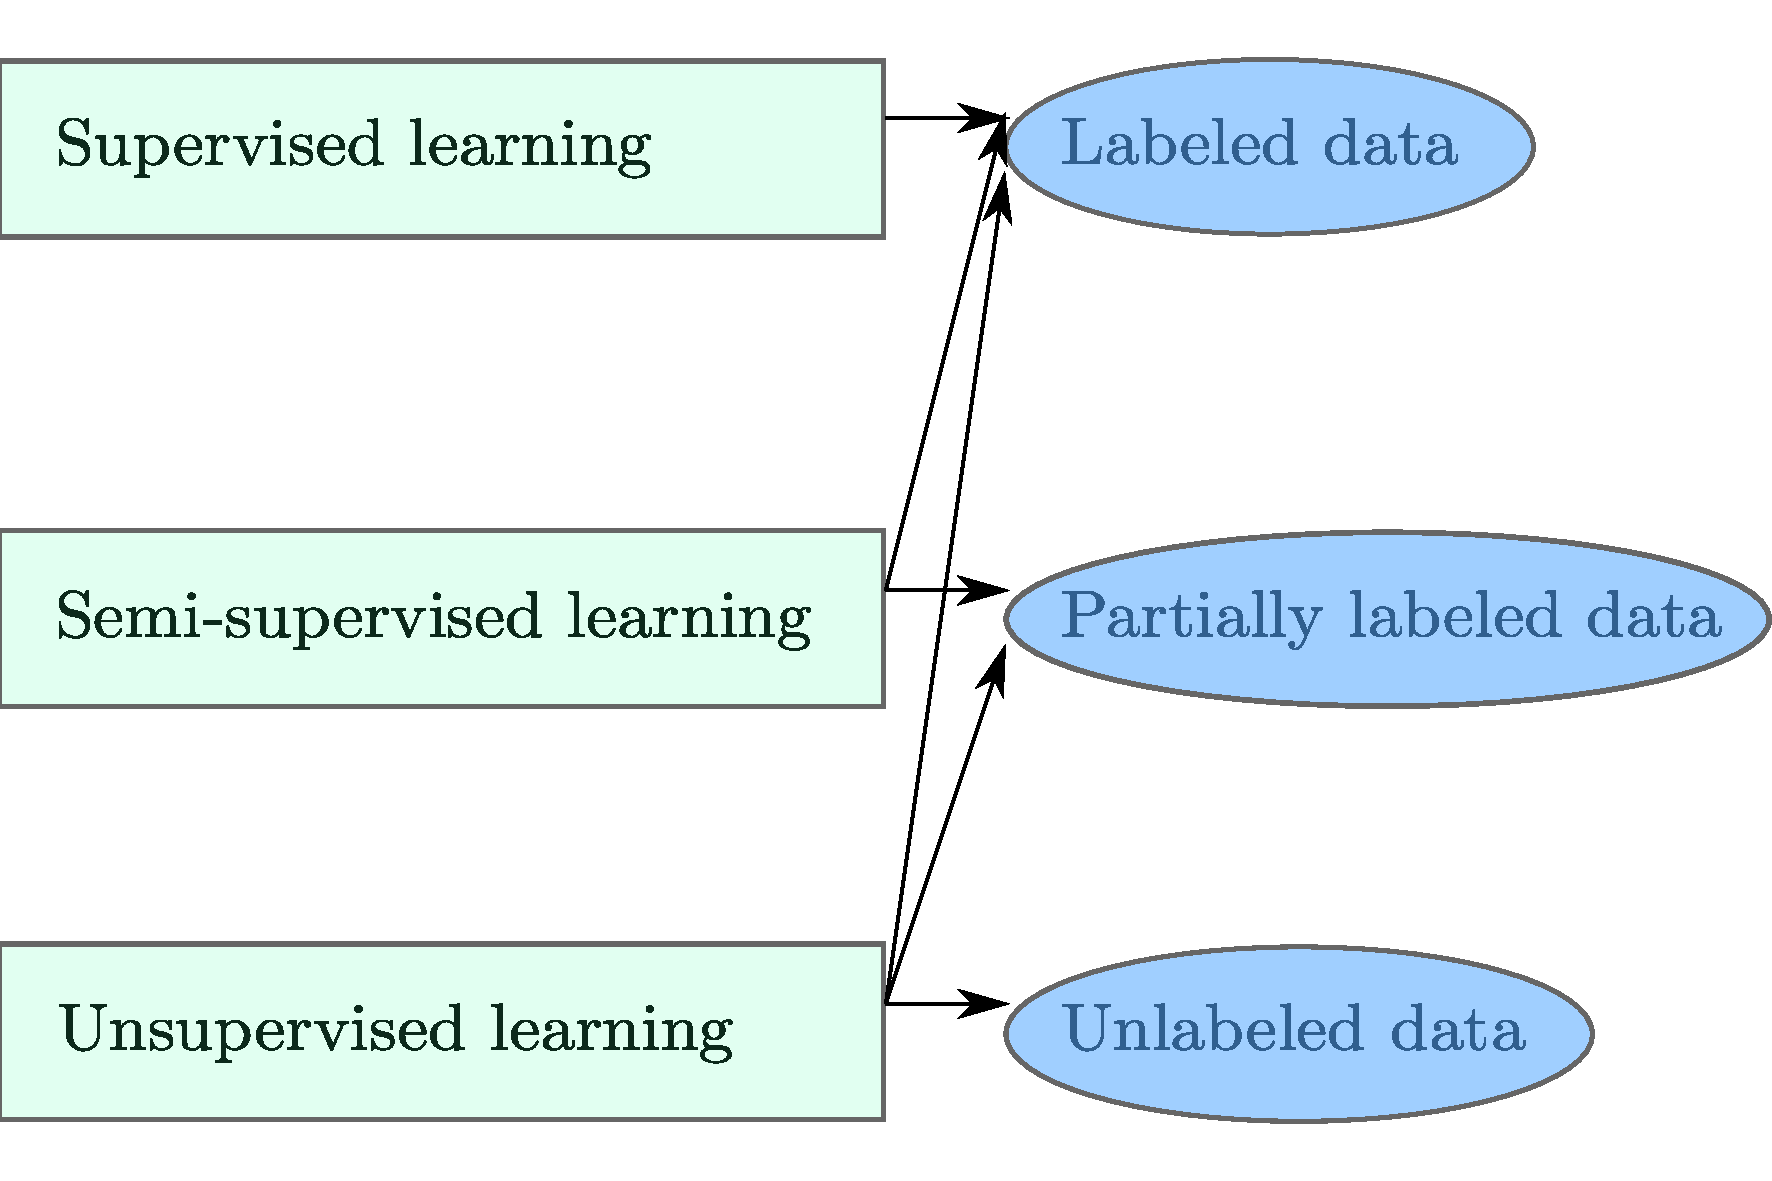
\includegraphics[width=\textwidth]{supersemiun.pdf}
    \caption{Levels of supervision in Machine Learning. Unsuperviesd algorithms are not dependent on labels and can therefore be applied on any type of data, whereas supervised algorithms require fully annotated data sets. Semi-supervised learning emerges as a middle ground between the two approaches.}
    \label{fig:supersemiun}
\end{figure}
Supervised learning can be seen as the problem of learning from data that is structured in pairs of patterns ($x$) and labels ($y$). The data set can consequently be represented as $S = {(x_1, y_1), ..., (x_n, y_n)}$. The task is then to predict the labels given the patterns. This transitions to semi-supervised learning when the training data does not necessarily contain labels for each pattern. The relations between the classes of supervision is illustrated in figure \ref{fig:supersemiun}. 

Methods for semi-supervised learning have shown success in improving the accuracy of supervised methods in settings where labeled data are limited \parencite{Zhou2012}. Generative models are well suited for semi-supervised learning, and several methods building on deep generative models have been proposed \parencite{kingma2014semi, salimans2016improved, springenberg2015unsupervised, wuliu2017selftrainsemisup, li2017triple}.

<<<<<<< HEAD
A common method for semi-supervised learning is self training. Self training is based on computing estimates of the missing labels which subsequently are reused for training the network. An interesting instance of self training when considering \acrshort{gans} is the triple \acrshort{gan} \parencite{li2017triple}. The triple \acrshort{gan} is a conditional \acrshort{gan} where the generator network is accompanied by a classifier network, which predicts the labels given the data. This network is also trained with and adversarial loss, at the same time as it is used to generate annotations for the generator. This constellation allows the networks to be trained on large amounts of unlabeled data when the classifier converges faster than the generator, which normally is the case.

The triple \acrshort{gan} is closesly related to the $\Delta$-\acrshort{gan} \parencite{triangleNIPS20177109} which also allows semi-supervised learning. The semi-supervised learning proposed for the $\Delta$-\acrshort{gan} is unlike the triple \acrshort{gan} not based on self training. Instead the objective function can be decomposed into a conditional part and a bidirectional part which can account for labeled and unlabeled data separately.
=======
A common method for semi-supervised learning is self training. Self training is based on computing estimates of the missing labels which subsequently are reused for training the network. An interesting instance of self training when considering \acrshort{gans} is the triple \acrshort{gan}, which is a conditional \acrshort{gan} where the generator network is accompanied by a classifier network, which predicts the labels given the data. This network is also trained with an adversarial loss, at the same time as it is used to generate annotations for the generator. This constellation allows the networks to be trained on large amounts of unlabeled data when the classifier converges faster than the generator, which normally is the case.
>>>>>>> 4886d906f95b333ed286f024e531f582fb58fd74

%\section{Image-to-Image Models}

%\section{Common architectures}

%\section{Normalization techniques}

%\section{Related work}
%Hmm, värt att nämna? 








\chapter{Methods}
Modelling annotated data: Normal GANs, image-to-image models.
Modelling partially annotated data: Triple-GAN.
\blindtext

\printbibliography[heading=bibintoc] % Print the bibliography (and make it appear in the table of contents)


\chapter{Results}

\chapter{Discussion}

\chapter{Conclusion}

% --------------------------------------------------------------------------------------------------------

\printbibliography[heading=bibintoc] % Print the bibliography (and make it appear in the table of contents)

\appendix

\chapter{Lots of images here}

\end{document}
